\documentclass[11pt,twocolumn]{asaproc}

\usepackage{graphicx}
\graphicspath{{images/}}

\usepackage{amsmath}
\usepackage{url}
\usepackage{numberedblock}

%\usepackage{mathtime}

%%UNCOMMENT following line if you have package
\usepackage{times}

\title{Bayesian Analysis of COVID-19 cases in California}

\author{Gulzina Kuttubekova\thanks{UCSC Baskin School of Engineering, Department of Statistical Science}}
\begin{document}


\maketitle





\begin{abstract} 
 Since mid-January of 2020, we have seen the first cases of coronavirus disease (COVID-19) in the US. Serious respiratory disease caused by the novel virus had taken the lives of approximately 400,000 people in the world and infected more than 6.7 million people worldwide. \url{https://www.worldometers.info/coronavirus/} provides various COVID-19 related statistics about the US as well.

% write what you will do here
We examine the dataset of COVID-19 cases in California. We are specifically interested in the number of infected people per county and if those numbers differ. We also look for a possible correlation between the number of infected people and the population density in each county. For an easier analysis, we used clustering (groups) of 58 counties in California provided by CA census. We employ four regression models to examine the infection rate and assess models by posterior predictive checks. 

% results - MODIFY 
A modified hierarchical model on the joint distribution of the number of infections and the number of deaths showed a better fit than the hierarchical model which doesn't take into account the mortality rate and its distribution. In general, we saw systematic differences in the number of deaths and infections across counties. The assumption that the mean number of the number of infections is 20\% of the population had a high impact on the posterior distribution in the first model.


\begin{keywords}
Bayesian regression analysis, COVID-19, hierarchical models, MCMC
\end{keywords}
\end{abstract}







\section{Introduction\label{Introduction}}

% Intro - motivation
 The novel virus is still spreading across the world despite the precautions taken by governments of different countries. The numbers connected to this pandemic are changing very rapidly, not every day, but every hour.  There are only 12 countries left where there are no officially confirmed cases of COVID-19, according to \url{https://www.aljazeera.com/news/}. However, it's believed that it's only a matter of time while the novel virus reaches those countries. Since the first massive cases of COVID-19 and related death numbers started increasing in the Greater Seattle area in the US in mid-March, the epicenter of outbreak shifted quickly from West to East coast. At the current time, the Greater New York area became the epicenter of coronavirus battle. Although the state of California has as twice as the population as New York state, according to Worldometers number of reported infected people in the New York area is seven times greater than in California. Obviously there are many external factors that can explain this discrepancy.
 
%Problem
We want to know if there exists any discrepancy in the distribution of COVID-19 cases among the counties in California. That discrepancy can be a result of different factors. For that reason, we used grouping information by CA census, s.t. 58 counties are grouped into based on like-mindedness of the counties, capacity of community-based organizations within the counties, and etc. We are also interested in the variation in the number of infected people by county. It's expected that as larger the population of the county as greater the number of infected people. Consequently, high the population density implies more number of infections. We would like to know if the population density has any effect on the infection rate, indeed. It might be a false expectation, since there are other factors influencing the infection rate as social culture, access to healthcare services and etc. 

%What we employ/do? 
We employ four regression models constructed in different ways. We tackle the problem stated above using a fully Bayesian approach. Results from those models are reported and compared. We also refer to results from the previous study, which are available at \url{https://github.com/kgulzina/} for additional model checks.




\subsection{Data}

% Describe dataset
We analyze the dataset which contains information about incidence and mortality due to coronavirus in California. The number of reported cases and death is given per each county as of 04/13/2020. There are 58 observations, as there are 58 counties in the state in total. There are 4 variables: \{County, Total.cases, Deaths, Population\} s.t. population, the number of infected people, and number of people who died from COVID-19 are given. Since we are interested in the number of infections and the number of infections is potentially overdispersed, we log-transform the count s.t. $y_{ij} = log(n_{ij})$, where $n_{ij}$ = is the number of cases for the $i^{th}$ county and $j^{th}$ region. Note that we added epsilon (fictitious one coronavirus case) for each county, as there are many counties with 0 observed cases in total. We treat $y_{ij}$ as a response variable. We also denote $c_{ij}$ which is the population. 

% additional datasets
We also use data set about population density of each county in California from \url{http://www.usa.com/rank/}. We denote population density as $d_{ij}$ for $i^{th}$ county and $j^{th}$ region. We also introduce new categorical variable \textit{region}, which indicates if county belongs to certain region.


\subsection{EDA}
The top three counties with the largest number of infected people are Los Angeles, San Diego, and Riverside.  Although San Francisco county has the largest population density $\sim18,553$, among all 58 counties in the state, it has 11 times less number of infected people compared to Los Angeles county with $\sim2,488$ population density. There are five counties that have zero reported cases of COVID-19. All five counties have population $\leq 32,000$. Interestingly four of those counties are in Northern California, and Mariposa county is relatively close to the highly populated county like Santa Clara. Up to date, $\sim 0.06\%$ of the population of California were infected with the virus. 

% include plot1: case numbers
\begin{figure}[t]
\centering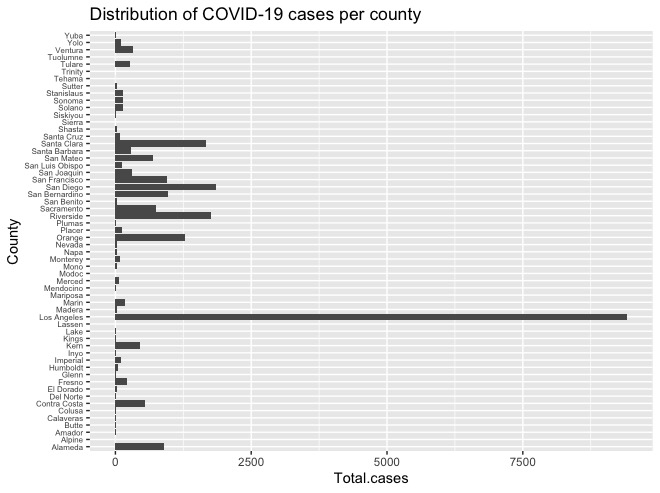
\includegraphics[scale=.30]{infected_per_county.jpeg}
\caption{Distribution of the total number of confirmed cases of COVID-19 across counties of California.}
\label{fig:totcases}
\end{figure}

% include plot2: case numbers by region
\begin{figure}[t]
\centering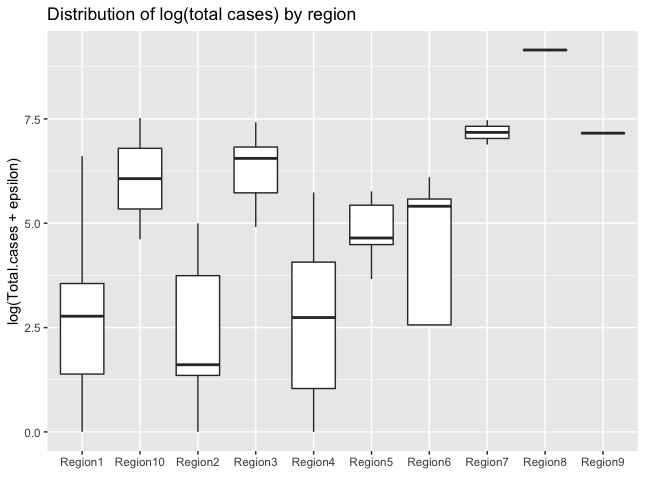
\includegraphics[scale=.31]{tot_cases_boxplot.jpeg}
\caption{Distributions of log-transformed coronavirus cases by region.}
\label{fig:boxplots}
\end{figure}

% talk about infection rate vs population
According to the plot in Figure ~\ref{fig:totcases}, we see that number of confirmed cases is not evenly distributed across counties. Los Angeles has the most noticeable spike in cases. The top five counties with the total number of infected people $\geq$ 1,000 are Los Angeles, San Diego, Riverside, Santa Clara, and Orange counties. Apparently these high numbers are associated with the population in each county. We also grouped 58 counties into 10 regions with the same characteristics. Figure \ref{fig:boxplots} shows that infection rates also differ significantly by region. Although the regions: 7, 8, and 9 have small variation (due to 1-2 observations in each group), their distribution noticeably differ from the rest of the regions.

% include plot3: scatter plot of density and total cases
\begin{figure}[t]
\centering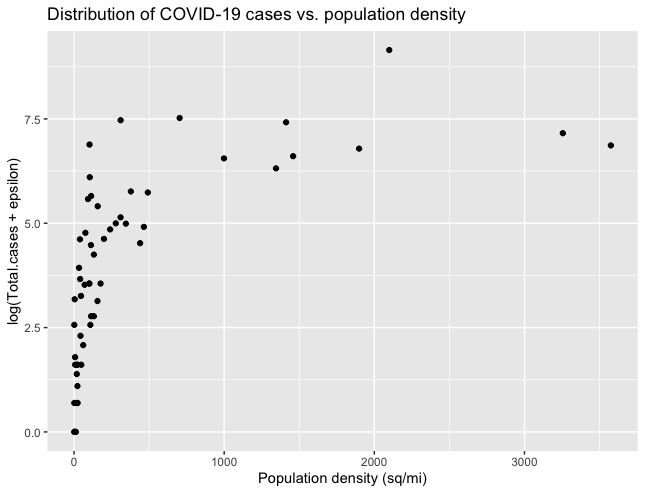
\includegraphics[scale=.31]{density_vs_totcases.jpeg}
\caption{Scatter plot of population density vs. total number of infections.}
\label{fig:densvstotcases}
\end{figure}

% talk about plot 3
Figure ~\ref{fig:densvstotcases} shows that as population density increases the number of infected people increases as well. There is some sort of nonlinear relationship between population density and log-transformed total number of infections. Note that we are interested in knowing if population density affects the distribution of COVID-19. Our hypothesis is also backed up with visual evidence provided in Figure ~\ref{fig:density}, the top 5 infected counties have population density of $\geq$ 1,000. Further, we investigate if the evidence we collected is enough to prove our hypothesis. Note that in the previous study we treated the number of confirmed cases $n_i$ as a known quantity, and now we treat it as a random variable of interest. 

% include plot4: population density of California counties
\begin{figure}[t]
\centering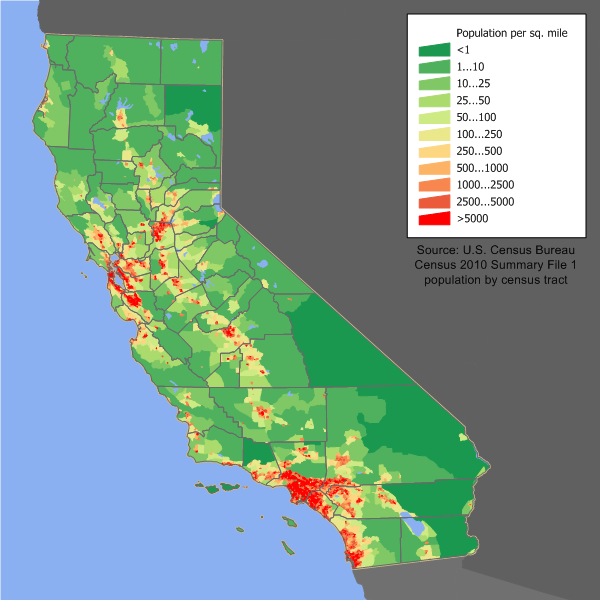
\includegraphics[scale=.30]{density.png}
\caption{Population density of California (Hines 2019).}
\label{fig:density}
\end{figure}

% preliminary findings
Our preliminary findings suggest that the distribution of total cases of coronavirus differ by counties, as well as by regions. There are some hypothetical factors affecting this discrepancy between counties. And we investigate further in what extent these factors are influential. For that purpose, we fit four models, which are described models in detail in the next section. 








\section{Methods}

% state the variables by detail
As stated before, $y_{ij}$ is log-transformed number of infections per county $i$ are independent observations from Normal distribution conditioning on $X \beta, c_{ij}, \sigma^2$. Also, population density of each county $d_{ij}$ is considered as an explanatory variable for modeling distribution of number of infections $log(n_{ij})$. 

% overall model
Throughout the study we consider the same structure of regression models:

$$Y = X \pmb{\beta}  + \epsilon$$ 

For county $i$ and region $j$, 

$$y_{ij} = \mathbf{x}_{ij}\pmb{\beta}  + \epsilon_{ij}$$

$$\epsilon_{ij} \sim N(0, \sigma^2  / \omega_{ij})$$

where errors are scaled with population factor $c_{ij}$ s.t. $\omega_{ij} = c_{ij} / 1000$. 

Note that structure of design matrix and parameter vector $\pmb{\beta} $ differ by model. We assume that $X$ and $c$ are fixed. Otherwise, we would have to account for uncertainty within covariates and set prior distirbution for each. Also, for convenience we set non-informative prior for each four model: $$ p(\pmb{\beta} , \sigma^2) \propto \frac{1}{\sigma^2}$$. Later, in order to compare models using Bayes factors we set G-priors for each model. It's given in model assessment section in full details. 

Since the overall structure does'n change for the same non-informative prior, the structure of posterior distribution is the same for all four models:

% overall posterior
Given the normal likelihood and non-informative prior, posterior becomes 

\begin{align*}
p(\pmb{\beta}, \sigma^2 | y, X) & = p(\pmb{\beta} | y, X, \sigma^2) p(\sigma^2 | y, X) \\
& \propto p(y | X\pmb{\beta}, \sigma^2) p(\pmb{\beta}, \sigma^2) \\
&\propto N(y | XB, \Sigma) \frac{1}{\sigma^2}
\end{align*}
 
 where $$\Sigma = \sigma^2 \Omega$$ $$\Omega = diag(1/\omega_{1,1}, 1/\omega_{1,2}, ..., 1/\omega_{10,1})$$
 
 Since we set non-informative prior, we know that posterior distribution of $\beta$ coincides with WLS estimates asymptotic distribution. I.e. 
 
 $$p(\pmb{\beta}| y, X, \sigma^2)  = N(\hat{\pmb{\beta}}, \sigma^2(X^{T}\Omega^{-1}X)^{-1})$$ is the WLS estimate of coefficient, where $\hat{\pmb{\beta}} = (X^T \Omega^{-1}X)^{-1} X^T  \Omega^{-1} y$. 
 
 Posterior marginal distribution of $\sigma^2$ is given as 
  $$p(\sigma^2 | y, X)  = IG (\frac{n-p}{2}, \frac{(n-p)\hat{\sigma^2}}{2})$$

where $p = $ \# of parameters in regression model, i.e. $p =$ rank(X). Note that $\sigma^2$ is also estimated using WLS method: $$\hat{\sigma}^2 = \frac{(y-X\hat{\pmb{\beta}})^T \Omega^{-1} (y-X\hat{\pmb{\beta}})}{n-p}$$   Here, $IG(\alpha, \gamma)$ = Inverse-Gamma$(\alpha, \gamma)$. 


% how to sample
\subsubsection{Sampling from posterior distribution}

Since overall structure of posterior is the same for all 4 models, sampling algorithms from joint posterior, as well as posterior predictive distributions is the same. Also since distributions are given in closed form, we can sample using \textit{factorization} and \textit{direct sampling}.

\vspace{5mm}

1. To sample from joint posterior:

\begin{itemize}
\item Sample $\sigma^2 \sim IG (\frac{n-p}{2}, \frac{(n-p)\hat{\sigma^2}}{2})$
\item Using $\sigma^2$, \\ sample $\pmb{\beta} \sim N(\hat{\pmb{\beta}}, \sigma^2(X^{T}\Omega^{-1}X)^{-1})$
\end{itemize}


2. To sample from posterior predictive distribution:

\begin{itemize}
\item Draw $\pmb{\beta}, \sigma^2$ from $p(\pmb{\beta}, \sigma^2 | Y, X)$
\item Draw $\tilde{y}$ from $\pmb{\beta} \sim N(\tilde{X}\pmb{\beta}, \sigma^2\Omega)$
\end{itemize}

Note that we actually know the closed form of posterior predictive distribution, which is given as: 

$$\tilde{y} \sim t_{v}(\tilde{X}\hat{\pmb{\beta}}, \hat{\sigma}^2(\Omega + \tilde{X}^T (X^T \Omega^{-1} X) ^{-1}\tilde{X}^T)$$ where degrees of freedom $v = n-p$. 

Although there is no difference if we sample $\tilde{y}'s$ using first approach or using analytically closed form, it's more convenient to sample from multivariate t-distribution. We proceed with the latter approach. 

% What will you do with results
After we obtain samples from joint posterior distribution, we report point and interval estimates of the posterior mean and posterior variance for each parameter. We also compare posterior mean of number of infections estimated by four models for ten counties from ten regions \{Placer, Humboldt, Santa Clara, Calaveras, Santa Barbara, Kings, San Bernardino, Los Angeles, Orange, San Diego\}. Note that counties from each region are chosen at random. 




% model 1
\subsection{Intercept only model}

First, we consider a model:
 
 % model construction
 Let $\beta = \mu$ s.t. there is one overall mean for all counties and regions. 
  
 % joint likelihood
 Then the model becomes $$y_{i} = \beta + \epsilon_{i} = \mu + \epsilon_{i} $$ for $i \in \{1, 2, ..., 58\}$.
 
 % sampling algorithm
 Other parts of the model except design matrix don't change, i.e. the posterior distribution structure and sampling algorithm are the same.
  
 
 


% model 2
\subsection{One factor regression model}

Now we add one factor to intercept model. We assume that infection rate in county depends on the population density of that county. Hence $\pmb{\beta} $ is modified as: 
 
 % model construction
 Let $\pmb{\beta} =  (\mu, \beta)$. The the model becomes 
 
 $$y_i = \mu + \beta d_{i} + \epsilon_{i}$$. Note that Design matrix now has two columns. 
 




% model 3
\subsection{Fixed effects model}

Thirdly, consider a model which assumes different groups means for ten regions. Mathematically, we consider different effect coefficient for each region along with one overall mean. Hence $\pmb{\beta} $ is modified as: 
 
 % model construction
Let $\pmb{\beta} =  (\mu, \eta_1, \eta_2, \eta_3, \eta_4)$. The the model becomes 
 
 $$y_{ij} = \mu + \eta_j + \epsilon_{ij}$$. Note that Design matrix now has five columns (but it's rank is 4). 
 




% model 4
\subsection{Fixed effects model (modified)}

Lastly, we consider a model which considers region-wise effect on the mean log(number of infections) as well as effect of population density. 
 
Hence $\pmb{\beta}$ is modified as: 
 
% model construction
 Let $\pmb{\beta} =  (\mu, \eta_1, \eta_2, \eta_3, \eta_4, \beta)$. The the model becomes 
 
 $$y_{ij} = \mu + \eta_j + \beta d_{ij} +  \epsilon_{ij}$$. Note that Design matrix now has six columns (but it's rank is 5). 
 




\subsection{Model assessment} % MODIFY

% compare models by posterior predictive distribution of LA county by 4 models
We also obtain samples of $\tilde{y}_{ij}$ from posterior predictive distribution, and compare its distribution predicted by 4 models. We chose the most populated county Los Angeles for this purpose. 

% compare first 4 models by R2
We also calculate $R^2 = 1 - \frac{SSE}{SST}$ of each model in order to compare them. Note that $R^2$ of model 1, i.e. $R^2_1 = 0$ since $SSE_1 = ||y-\hat{y}_1||^2 = SST$. It would be more appropriate to compare models by another measure, for instance Bayes factor. Since we can't get nice form of Bayes factor with non-informative priors, we re\-run all four models with G\-priors. 

% what does G-prior mean  MODIFY - Maybe you will need it or nooot IDK
\subsubsection{Regression models with Zellner's G-prior}

Regression models with G-priors are given in the following form:

$$p(Y | X, \beta, \sigma^2) = N(Y | \pmb{\mu} + X\beta, \sigma^2)$$

$$ $$



% Bayes factors with G-priors
Then we have Bayes factor of the form: 

\begin{align*}
BF_{1,2} & = \frac{p(y | M1, g)}{p(y | M2, g)} \\
&= (1+g)^{\frac{p2-p1}{2}}\Big(\frac{(1+g(1-R^2_{m2}))}{(1+g(1-R^2_{m1}))}\Big)^{\frac{n-1}{2}}
\end{align*}

where $g$ is a constant which comes from G-prior. M1 is the model 1 with R-square: $R^2_{m1}$ and $p1 = rank(X_1)$. Similarly $R^2_{m2}$ is R-square measure of model 2 and $p2 = rank(X_2)$. 

% how do we choose value of g: - MODIFY


% hypothesis testing
\subsubsection{Hypothesis testing}
We are interested in Bayes Factors, since we want to test the hypotheses as: 

$$1. \hspace{2mm} H_0: \eta_1 = \eta_2 = ... = \eta_5$$ In other words we want to know if the grouping is significant and worth considering. 

$$2. \hspace{2mm} H_0: \beta = 0$$ In other words, we want to test if population density if significant enough and worth considering. 

Note that these hypothesis can be tested using different methods, such as by comparing models posterior predictive performance or by comparing posterior distributions of parameters as we did later in the analysis. 









\section{Analysis} % - MODIFY

% model 1
\subsection{Intercept only model}

% posterior of mu, sigma2
\begin{figure}[t]
\centering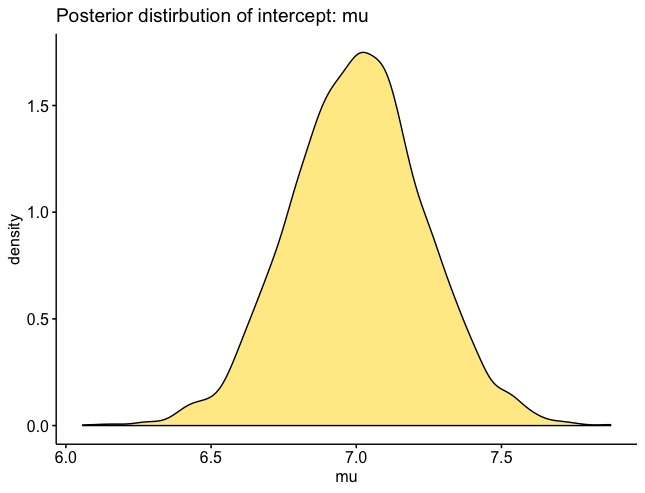
\includegraphics[scale=.30]{interceptM1.jpeg}
\caption{Posterior distribution of : $\alpha$ and $\beta$ parameters}
\label{fig:intercept}
\end{figure}

% posterior of sigma2's for 4 models
\begin{figure}[t]
\centering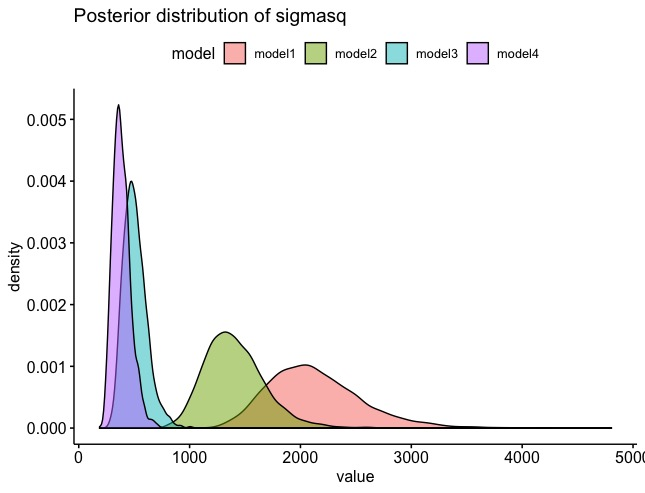
\includegraphics[scale=.30]{sigmasq.jpeg}
\caption{Posterior distributions of $\sigma^2$ by all four models}
\label{fig:sigmas}
\end{figure}

We obtain 5,000 sample draws from joint posterior distribution of $\beta, \sigma^2$. As wee see in Figure \ref{fig:intercept} the posterior distribution of $\mu$ is updated from flat prior and concentrated around the WLS estimate. 95\% Confidence intervals for each parameter are given as: $E[\mu | Y]$ is in [6.558, 7.457], $E[\sigma^2 | Y]$ lies between [1465.277, 3100.122]. Note that we allowed heteroskedasticity i.e. we assumed that errors are not identically distributed. We started from the simplest null model and added factors one by one. As we added factors, estimated range of $\sigma^2$ squeezed, as can be seen from Figure \ref{fig:sigmas}. Also, if we compare the OLS estimate of $\mu$ when we assume iid errors and MAP estimate of $\mu$ with weighted errors, we see that $\hat{\mu}_{OLS} = 3.868$ and $\hat{\mu}_{MAP} = 7.006$. By transforming the estimates back to $n_{ij}$ scale, we have OLS estimate of mean total number of infections = 47 and MAP estimate = 1102. There is huge discrepancy between the estimates. It's expected since the model doesn't include any factors and errors are indeed weighted rather than identically distributed. 




% model 2 
\subsection{One factor regression model}

We obtain 5,000 sample draws from joint posterior distribution of $\mu, \beta$ and $\sigma^2$. Posterior distribution of $\sigma2$ is given in Figure \ref{fig:sigmas}. As we see the center of distribution shifted to the left (decreased) and range became shorter. MAP estimates of parameters in model 2 are given as $\hat{\mu}_{MAP} = 5.74$, $\hat{\sigma}^2_{MAP} = 1375.77$ and $\hat{\beta}_{MAP} = 0.00098$. Confidence interval for $\sigma^2$ is given as [973.453, 2044.204]. We compare posterior expected number of infections for different regions in Tables \ref{tab:infections} and \ref{tab:infectionss}. Since this model considers population density as a factor, prediction of total number of infections is mainly dictated by the value of that density. For instance, model 2 overestimated the total number of infections in Orange county as larger than of Los Angeles county, because it has higher population density than Los Angeles county.




% model 3
\subsection{Fixed effects model}

We obtain 5,000 sample draws from joint posterior distribution of $\mu, \eta_1, \eta_2, ..., \eta_{10}$ and $\sigma^2$. If we compare posterior distribution of $\sigma^2$ in Figure \ref{fig:sigmas}, we see that it's more peaked and shrunk . Confidence interval for $\sigma^2$ is given as [338.809, 759.904].  As expected, the interval estimate of $\sigma^2$ is shorter than interval estimates from previous models. We also compare posterior expected number of infections for one county from each 10 regions in Tables \ref{tab:infections} and \ref{tab:infectionss}. Estimates are stabilized for some counties, but the model is still overestimating number of infections for counties with relatively smaller population. 




% model 4
\subsection{Fixed effects model (modified)}

We obtain 5,000 sample draws from  joint posterior distribution of $\mu, \beta, \eta_1, \eta_2, ..., \eta_{10}$ and $\sigma^2$. The 95\% confidence interval for $\sigma^2$ is given as [275.467, 580.585]. As also noted in Figure \ref{fig:sigmas} estimate value of $\sigma^2$ has decreased as we added more factors to the model. We also compare posterior expected number of infections for one county from each 10 regions in Tables \ref{tab:infections} and \ref{tab:infectionss}.  Although $\sigma^2$ decreased as we added multiple factors to the model, we see that model still underestimates number of infections for counties like Santa Clara, Santa Barbara. It's also still overestimating number of infections for counties with relatively smaller population. 





% comparing models - MODIFY
\subsection{Comparing the models}

We fit four regression models in total to the COVID-19 data. To account for potential overdispersion and zero-inflated dataset, we add some epsilon (=1) and log-transform the total number of cases and treat it as a response variable.

% report posterior expected number of infections in 10 counties by first model and real data
\begin{table}
\caption{Expected number of infections predicted by model 1 for 10 counties from 10 different regions.}
\label{tab:infections}
\begin{center}
\begin{tabular}{ccccc}
\hline
\hline
\\[-5pt]
\multicolumn{1}{c}{County} &
\multicolumn{1}{c}{observed} &
\multicolumn{1}{c}{M1}\\
\hline
Placer&	127&   7\\
Humboldt&     50&  7 \\
Santa Clara&	1,666& 7\\
Calaveras&     9&  7\\
Santa Barbara&     284& 7\\
Kings&     12& 7\\
San Bernardino&     977& 7\\
Los Angeles&     9,420& 7\\
Orange&     1,283& 7\\
San Diego&     1,847& 7\\
\hline
\end{tabular}
\end{center}
\end{table}


% report posterior expected number of infections in 10 counties by 3 models

\begin{table}
\caption{Expected number of infections predicted by models 2-4 for 10 counties from 10 different regions.}
\label{tab:infectionss}
\begin{center}
\begin{tabular}{ccccc}
\hline
\hline
\\[-5pt]
\multicolumn{1}{c}{County} &
\multicolumn{1}{c}{M2} &
\multicolumn{1}{c}{M3} &
\multicolumn{1}{c}{M4}\\
\hline
Placer&	396&   141 & 86\\
Humboldt&     323&  50 &	 44\\
Santa Clara&	1,243& 801	& 648\\
Calaveras&     326&  111 & 85\\
Santa Barbara&     349& 176 & 159\\
Kings&     348& 243 & 238\\
San Bernardino&     346& 1,330 & 1,199\\
Los Angeles&     2,432& 9,384 & 9,423\\
Orange&     7,518& 1,284 & 1,280\\
San Diego&     622& 1,605 & 1,636\\
\hline
\end{tabular}
\end{center}
\end{table}

% comment on the posterior of sigmas above
As expected, as we increase complexity of the model, the posterior distribution of $\sigma^2$ is more concentrated and has shorter range width. There is noticeable difference when we add population density or region factor to the model, however there isn't much difference when we proceed from model 3 to model 4. It might suggest that given region information, the population density is not that significant in estimating the number of infections. 


% comment on the table above
From Tables \ref{tab:infections} and \ref{tab:infectionss} we see that the worst model among four is the intercept model which considers the same mean for all counties i.e. pools everything together, and doesn't take any external factors into account. It predicts the same value: total number of infections = 7 for all counties. The second model, with density population as a covariate, showed better results, but still overestimated or underestimated most of the observations. There is a slight change in predictions between model 3 and model 4, which also suggests that population density isn't that worth considering when we are given region information. 



% plot with checks
\begin{figure}[t]
\centering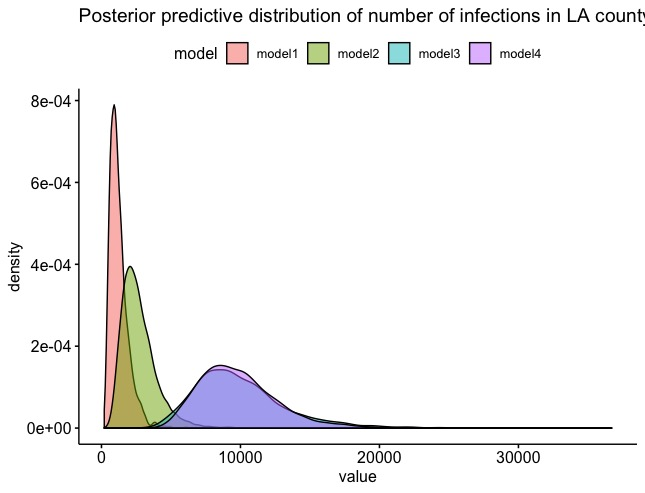
\includegraphics[scale=.30]{LA.jpeg}
\caption{Distribution of number of infections in Los Angeles county estimated by model 1-4.}
\label{fig:LA}
\end{figure}



% Model checks - draw samples from posterior predictive distribution
We noticed in EDA that Los Angeles county has the largest proportion of infections across counties in California. So we draw 5,000 samples from the posterior predictive distribution of $y_{i,j}$ for Los Angeles county. As we see from Figure \ref{fig:LA} estimates are stabilized for models 3 and 4. Actually, there is almost no difference in posterior predictive distributions generated by model 3 and 4. It agains suggests that reduced model with region as factor performs as good as full model. Note that true observed value is 9,420 infections and both models 1 and 2 underestimated that value. 
 

% overall computational performance
There wasn't much difference in the computation time of the models for obtaining samples from joint posterior and posterior predictive distribution. This is because we have all posterior distributions in closed form and we can directly sample from them. 


% compare R-squares with non-informative prior - MODIFY
\begin{table}
\caption{$R^2$ measure of models w.r.t. different priors.}
\label{tab:infectionss}
\begin{center}
\begin{tabular}{ccccc}
\hline
\hline
\\[-5pt]
\multicolumn{1}{c}{Prior} &
\multicolumn{1}{c}{M1} &
\multicolumn{1}{c}{M2} &
\multicolumn{1}{c}{M3} &
\multicolumn{1}{c}{M4}\\
\hline
$1/\sigma^2$ &	0&   0.410 & 0.656 & 0.742\\
g-prior &	396&   141 & 86 & h\\
\hline
\end{tabular}
\end{center}
\end{table}


% comment on R2's - MODIFY
As expected, $R^2$ increases as we include more factors to the model. If the variation in $y$ explained by regression model increases by almost \%41 when we added population density and by \%65.6 when we added region covariates. However, when we add population density given the region information, that percentage increase only by ~\%8. 



% compare Bayes factors with g-priors - MODIFY










\section{Discussion} % - MODIFY

% intro
We employed four different constructions of regression model. We treated the number of infected people as a random variable. Our preliminary results showed that the infection rate across counties is not homogenous. It was also confirmed throughout by fitting the models above. 

% was it worth to add region? population density? - MODIFY (Bayes factors???)
As we see from the analysis above, it's both worth considering region information and population density to the model. Both of those factors were successful in some extent in explaining the variation in the number of infections in California. However, if it's worth considering both factors at the same time is under doubt, since we couldn't see much difference when comparing performances of model 3 and 4. Obviously the more factors you add, it's always better for the model, from mathematical point of view. In practice it doesn't always work that way. At this point, since we get those covariates for granted (population density and region information from US census bureau), it's worth adding them both. For future, we may want to add more covariates as we see there is still room for improvement. In that case we'll have to reconsider our choice of factors since some of them might be correlated and carry the same information. 


% is there other models to consider/factors to add? - MODIFY



% Talk about future: time when will we reach that 20%, how to slow the spread and find the patterns in different counties
In this analysis we ignored the time feature of the spread of the virus. So it can be the next step to include time in our model, i.e consider time series model. 

% Time-space varying parameter
As a next step, we can consider a model that accounts for the time and space varying nature of the spread of the virus. I.e we might want to employ Gaussian or Poisson processes that are suitable for time series as well as spatial data. 




%Note:BibTeX also works - MODIFY

\begin{references}
\itemsep=0pt
{\footnotesize

\item
Aljazeera, News
\\\url{https://www.aljazeera.com/news/}

\item
Hines B 2019, Population Density of California
\\\url{https://storymaps.arcgis.com/stories/252b65cbe331420389c61453c61ea221}

\item
Kuttubekova G 2020, Bayesian Analysis of COVID-19 cases in California
\\\url{https://github.com/kgulzina/bayesian-analysis-of-COVID19-in-CA}

\item 
Worldometer: Coronavirus,
\\\url{https://www.worldometers.info/coronavirus/}


\item 
Gelman, A., Carlin, J. B., Stern, H. S., Dunson, D. B., Vehtari, A., \& Rubin, D. B. (2013), $\textit{Bayesian Data Analysis} (3^{rd}$ ed.). CRC Press. Taylor \& Francis Group.

% add dataset resources!!!! 


}
\end{references}


\end{document}


